\documentclass[11pt]{article}
\usepackage[toc,page]{appendix}
\usepackage{amsmath, amssymb}
\usepackage[utf8]{inputenc}
\usepackage[T1]{fontenc}
\usepackage[style=apa,backend=biber]{biblatex}
%\usepackage{biblatex}
\addbibresource{references.bib}
\usepackage{graphicx}
\usepackage{tikz}
\usetikzlibrary{automata,positioning,shapes.geometric, arrows.meta, fit, backgrounds, calc, chains}
\graphicspath{./images/Easy_Pictures/SMR_MULT_Repackaging}%\usepackage{kpfonts}
\usepackage{float}
\usepackage[margin=1in]{geometry}
\usepackage{cancel}
\usepackage{epsfig}
\usepackage{tikz-3dplot}
\usepackage{darkmode}
\usepackage{dirtytalk}
\usepackage{longtable,booktabs,array}
\usepackage{calc} % for calculating minipage widths
\usepackage[utf8]{inputenc}
\usepackage[T1]{fontenc}
\usepackage{xcolor}
\usepackage{listings}


\usepackage{etoolbox}
\usepackage{hyperref}
\hypersetup{
 colorlinks=true,
 linkcolor=blue,
 filecolor=magenta, 
 urlcolor=cyan,
 pdftitle={Hermeneutic Calculator},
 citecolor=blue,
 }


\urlstyle{same}

\lstdefinestyle{htmlStyle}{
 language=HTML,
 basicstyle=\ttfamily\small,
 keywordstyle=\color{blue}\bfseries,
 commentstyle=\color{gray}\itshape,
 stringstyle=\color{red},
 breaklines=true,
 frame=single,
 numbers=left,
 numberstyle=\tiny\color{gray},
 columns=fullflexible,
}
\lstdefinelanguage{HTML}{
 keywords={<!DOCTYPE, html, head, title, body, h1, h2, h3, p, div, span, a, img, ul, li, table, tr, td, th, style, link, script},
 sensitive=true,
 comment=[l]{//},
 morecomment=[s]{/*}{*/},
 morestring=[b]',
 morestring=[b]"
}
\lstset{style=htmlstyle, language=html}
% Updated to explicitly pass the language option
%\lstinputlisting[style=htmlstyle, language=html]{./html/example.html}
%\usepackage{tocloft}

% Optional: define some custom colors
\definecolor{sliceRed}{RGB}{225,224,91} % matching "varyellow" from your code
\definecolor{linkYellow}{RGB}{255,215,0} % a golden yellow
\tdplotsetmaincoords{70}{110}

\title{Subtraction Strategies: Decomposition}
\author{Compiled by: Theodore M. Savich}

\begin{document}
\maketitle
\subsection*{Transcript}
Video from \textcite{Carpenter1999}. Strategy descriptions and examples adapted from \textcite{HackenbergCourseNotes}
\begin{itemize}
      \item \textbf{Teacher:} Lucy ordered 45 cupcakes for her birthday. At the party, her guests ate 27 cupcakes, how many cupcakes did she have left? [BACKGROUND] 
      \item \textbf{Joel:} This is 10, this is 10, this is 10, this is 10 and this is five.18. 
      \item \textbf{Teacher:} Explain to us what you did there. 
      \item \textbf{Joel:} I have, this is 10, this is 10, this is 10, and this is five. So I take away 20 and I take away five. I take away two more. So they enter and then I counted these and those, and so the answer was 18. 
      \item \textbf{Teacher:} Nice work
\end{itemize}
 
\noindent \textbf{Notation Representing Joel's Solution:}
\begin{align*}
      47-27 & \\
      45 - 20 &=25 \\
      25 - 7 &= ?\\
      &2 \text{ tens } + 5 \text{ ones } - 7 \text{ ones } \\
      1 \text{ ten } + &1 \text{ ten } + 5 \text{ ones } - 7 \text{ ones } \\
                             &\downarrow \text{DECOMPOSE}\\
      1 \text{ ten } + &10 \text{ ones }+5 \text{ ones } - 7 \text{ ones } \\ 
      &1 \text{ ten } + 8 \text{ ones }+\underbrace{7 \text{ ones }- 7 \text{ ones }}_{=0}\\ 
      %									&=0 \\
      &1 \text{ ten } + 8 \text{ ones } 
      \end{align*}
      

      \includegraphics[width=.8\textwidth]{images/Easy_Pictures/SAR_SUB_Decomposition/PDF/SAR_SUB_Decomposition.pdf}

      \noindent \textbf{Notation Representing Joel's Solution:}
      \noindent Imagine representing both numbers by their base units and ones. Begin by subtracting the base components, then subtract the ones. If there aren't enough ones available in the larger number to subtract the ones from the smaller number (while keeping the result positive), break one base unit into its individual ones. Finally, remove only the exact number of ones required to complete the subtraction.


\subsection*{Decomposition}

\subsubsection*{Description of Strategy}
\begin{itemize}
    \item \textbf{Objective:} Decompose a base unit from the minuend into ones to have enough ones to subtract the ones in the subtrahend.
\end{itemize}

\subsubsection*{Automaton Type}
\textbf{Pushdown Automaton (PDA)}: Needed to handle the decomposition process and keep track of base units.

\subsubsection*{Formal Description of the Automaton}

We define the PDA as the 7-tuple
\[
M = (Q,\,\Sigma,\,\Gamma,\,\delta,\,q_{0/accept},\,Z_0,\,F)
\]
where:
\begin{itemize}
    \item \(Q = \{q_{0/accept},\, q_1,\, q_2,\, q_3,\, q_4,\, q_5\}\) is the set of states.
    \item \(\Sigma = \{0,1,2,3,4,5,6,7,8,9\}\) is the input alphabet.
    \item \(\Gamma = \{Z_0\} \cup \{b \mid b \in \mathbb{N}\}\) is the stack alphabet, where \(Z_0\) is the initial stack symbol and \(b\) represents a base unit (e.g., 10 in base-ten).
    \item \(q_{0/accept}\) is the start state, which is also the accept state.
    \item \(F = \{q_{0/accept}\}\) is the set of accepting states.
\end{itemize}

The transition function \(\delta\) is defined as:
\begin{enumerate}
    \item \(\delta(q_{0/accept},\, \text{``}M,S\text{''},\, Z_0) = \{(q_1,\, Z_0)\}\) \\
          (Split the minuend \(M\) and subtrahend \(S\) into their base and ones components.)
    \item \(\delta(q_1,\, \varepsilon,\, Z_0) = \{(q_2,\, Z_0)\}\) \\
          (Compare the ones in \(M\) and \(S\).)
    \item \(\delta(q_2,\, \varepsilon,\, Z_0) = \{(q_3,\, b\,Z_0)\}\) \\
          (If the ones in \(M\) are insufficient, decompose a base unit \(b\) into ones.)
    \item \(\delta(q_2,\, \varepsilon,\, Z_0) = \{(q_4,\, Z_0)\}\) \\
          (If the ones in \(M\) are sufficient, proceed to subtract ones.)
    \item \(\delta(q_3,\, \varepsilon,\, b) = \{(q_4,\, b)\}\) \\
          (After decomposition, subtract the ones.)
    \item \(\delta(q_4,\, \varepsilon,\, Z_0) = \{(q_5,\, Z_0)\}\) \\
          (Subtract the bases.)
    \item \(\delta(q_5,\, \varepsilon,\, Z_0) = \{(q_{0/accept},\, Z_0)\}\) \\
          (Output the final difference.)
\end{enumerate}

\subsubsection*{Automaton Diagram for Decomposition}

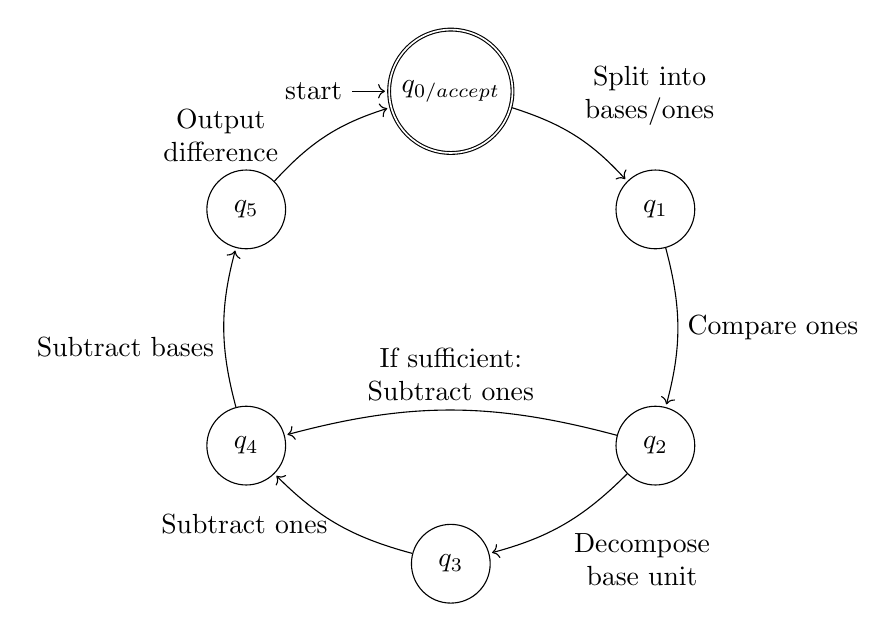
\begin{tikzpicture}[
    shorten >=1pt,
    auto,
    node distance=3cm,
    every state/.style={minimum size=1cm}
]
    % Arrange 6 states on a circle:
    % q_{0/accept} at 90°, q_1 at 30°, q_2 at -30°, q_3 at -90°, q_4 at -150°, q_5 at 150°.
    \node[state, initial, accepting] (q0) at (90:3cm) {$q_{0/accept}$};
    \node[state] (q1) at (30:3cm) {$q_1$};
    \node[state] (q2) at (-30:3cm) {$q_2$};
    \node[state] (q3) at (-90:3cm) {$q_3$};
    \node[state] (q4) at (-150:3cm) {$q_4$};
    \node[state] (q5) at (150:3cm) {$q_5$};

    % Transitions with non-overlapping labels:
    \path[->]
        (q0) edge[bend left=15] node[above right, align=center] {Split into\\bases/ones} (q1)
        (q1) edge[bend left=15] node[right, align=center] {Compare ones} (q2)
        (q2) edge[bend left=15] node[below right, align=center] {Decompose\\base unit} (q3)
        (q2) edge[bend right=15] node[above, align=center] {If sufficient:\\Subtract ones} (q4)
        (q3) edge[bend left=15] node[left, align=center] {Subtract ones} (q4)
        (q4) edge[bend left=15] node[below left, align=center] {Subtract bases} (q5)
        (q5) edge[bend left=15] node[left=14pt, align=center] {Output\\difference} (q0);
\end{tikzpicture}

\clearpage
\subsubsection*{HTML Implementation}
\lstinputlisting[style=htmlStyle, language=html]{./new_html/SAR_SUB_DECOMPOSITION.html}

\printbibliography

\end{document}